
\documentclass[12pt,letterpaper]{report}
\usepackage{bbm}
\usepackage{dsfont}
\usepackage{multicol}
\usepackage{lipsum}
\usepackage{mwe}
\usepackage{graphicx}
\usepackage{epstopdf}
\epstopdfsetup{outdir=./}
\usepackage{subcaption}
\usepackage{geometry}
\usepackage{float}
\usepackage{amsmath,amssymb}
\usepackage{makecell}
\usepackage{lmodern}
\usepackage{mathtools}
\usepackage[thinc]{esdiff}
\usepackage{import}
\usepackage{braket}
\DeclarePairedDelimiter{\ceil}{\lceil}{\rceil}

\newcommand{\lam}{\lambda}

% Title Page
\title{ Dynamique moléculaire et simulation Monte-Carlo \\ 3: Monte Carlo Simulations and the Photon Gas}
\author{Bruno Rodriguez Carrillo \\ EPFL}

\geometry{
	a4paper,
	total={185mm,260mm},
	left=15mm,
	top=15mm,
}

\begin{document}	
	\maketitle
	% theory questions
	%### Monte Carlo and Statistical Mechanics
	
	\begin{enumerate}
		\item 
		Show that based on the form of the Hamiltonian: 
		$$
		\begin{aligned}
		\mathrm{H} = \mathrm{T}(\mathbf{p}) + \mathrm{V}(\mathbf{q}),
		\end{aligned}
		$$
		
		the partition function can be divided into a kinetic and potential
		part, and for an ensemble average of an observable $O(\mathbf{q})$
		that depends on $\mathbf{q}$ only, one has: 
		
		$$
		\begin{aligned}
		\left<O(\mathbf{q})\right> &= \frac{\int_\Gamma O(\Gamma)e^{-\beta E(\Gamma)} \mathrm{d}\Gamma}{\int_\Gamma e^{-\beta E(\Gamma)} \mathrm{d}\Gamma} \\
		&= \frac{\int O(\mathbf{q})e^{-\beta V(\mathbf{q})} \mathrm{d}\mathbf{q}}{\int e^{-\beta V(\mathbf{q})} \mathrm{d}\mathbf{q}},
		\end{aligned}
		$$
		
		which is the equation you have encountered in the section on detailed balance.
		
		We know that the partition function is: $Z = \int_{\Gamma(\mathbf{p}, \mathbf{q})} e^{-\beta E(\Gamma)} \mathrm{d}\Gamma(\mathbf{p}, \mathbf{q})$, with $\Gamma(\mathbf{p}, \mathbf{q})$ the configuration space spanned by momenta $\mathbf{q}$ and velocities $\mathbf{q}$.
		
		Now, if we have that the Hamiltonian is given by $\mathrm{H} = \mathrm{T}(\mathbf{p}) + \mathrm{V}(\mathbf{q})$ and kinetic and potential energies are not couple, then we can split the partition function $Z$ into: 
		
		$$
		Z = \int_{\Gamma(\mathbf{p}, \mathbf{q})} e^{-\beta ( \mathrm{T}(\mathbf{p}) + \mathrm{V}(\mathbf{q}) )  } \mathrm{d}\Gamma(\mathbf{p}, \mathbf{q}) = 
		\int_{\Gamma(\mathbf{p}, \mathbf{q})} e^{-\beta \mathrm{T}(\mathbf{p})  } \mathrm{d}\mathbf{p}
		\cdot
		e^{-\beta \mathrm{V}(\mathbf{q} ) } \mathrm{d} \mathbf{q}
		$$
		
		Now, if we want to compute the average value of an observable $\left<O(\mathbf{q})\right>$, we have: 
		$$
		\left<O(\mathbf{q})\right> = 
		\dfrac
		{			
			\int_{\Gamma(\mathbf{p}, \mathbf{q})} \left<O(\mathbf{q})\right> \cdot  e^{-\beta \mathrm{T}(\mathbf{p})  } \mathrm{d}\mathbf{p}
			\cdot
			e^{-\beta \mathrm{V}(\mathbf{q} ) } \mathrm{d} \mathbf{q}
		}
		{
			\int_{\Gamma(\mathbf{p}, \mathbf{q})} e^{-\beta \mathrm{T}(\mathbf{p})  } \mathrm{d}\mathbf{p}
			\cdot
			e^{-\beta \mathrm{V}(\mathbf{q} ) } \mathrm{d} \mathbf{q}
		} 
		= 
		\dfrac
		{			
			\int_{\Gamma(\mathbf{p}, \mathbf{q})} \left<O(\mathbf{q})\right>
			\cdot
			e^{-\beta \mathrm{V}(\mathbf{q} ) } \mathrm{d} \mathbf{q}
		}
		{
			\int_{\Gamma(\mathbf{p}, \mathbf{q})} 
			e^{-\beta \mathrm{V}(\mathbf{q} ) } \mathrm{d} \mathbf{q}
		} 		
		$$
		
		where we have used the fact that $O(\mathbf{q}) $ is a function of $\mathbf{q}$ only and as such, the term $e^{-\beta \mathrm{T}(\mathbf{p} ) }$ can be taken out of the integral. 
		
		\item 
		**Bonus:** In the Metropolis scheme, why is it important that $P^\prime$ be a symmetric matrix?
				
		Based on (XXX), we have:
		
		Let us introduce the function $\rho (X, t)$ which gives us the probability of occurrence of configuration $X$ at time $t$ (for an ergodic chain, $\rho (X, t)$ becomes independent of $t$ for large $t$). The change in this function from one step to another is governed by two processes: (i) going from a configuration $X$ at time $t$ to some other configuration $X^\prime$ at $t + 1$, leading to a decrease of $\rho (X)$, and (ii) going from some configuration $X^\prime$ at time $t$ to $X$ at time $t + 1$, thus causing an increase in $\rho (X)$.	Then we have the following formula:
		
		$$
		\rho (X, t + 1) - \rho (X, t) = -\sum_{X^\prime}^{}T(X \rightarrow X^\prime )\rho (X, t) + 
		\sum_{X^\prime}^{}T(X^\prime \rightarrow X )\rho (X^\prime , t)		
		$$
		
		Since we try to find the invariant distribution, this condition is fulfilled when $\rho (X, t + 1) = \rho (X, t)$ and then:

		$$
		\sum_{X^\prime}^{}T(X \rightarrow X^\prime )\rho (X, t) = 
		\sum_{X^\prime}^{}T(X^\prime \rightarrow X )\rho (X^\prime , t)		
		$$
		
		Such expression corresponds to the detailed balance solution. Such equation makes sure that the 'rates' from and to state $X$ or $X^\prime$ are balanced. We can expand this and state that for any pair of states $(X, X^\prime)$ the number of particles is balanced. 
		
		Additionally, we have express $T$ as a product of two quantities:
		$T(X \rightarrow X^\prime ) = \omega_{XX^\prime} \cdot A_{XX^\prime}$
		
		Hence: 
		$$
		\sum_{X^\prime}^{} \omega_{XX^\prime} \cdot A_{XX^\prime}  \rho (X, t) = 
		\sum_{X^\prime}^{} \omega_{X^\prime X} \cdot A_{X^\prime X} \rho (X^\prime , t)		
		$$
		
		Such detailed balance is fulfilled when $\omega_{XX^\prime}=\omega_{X^\prime X}$. This corresponds to the matrix $P'$.
		
		When the transition probability matrix $P^\prime$ is symmetric, our system has reached the desired distribution, also known as invariant distribution, and then we can compute the average value of an observable quantity $\left<O\right>$. This means that if $P^\prime$ is a symmetric matrix, the probability of going from a new state to an old one is the same as going from an old state to a new one.
		
	\end{enumerate}

	\section*{The Photon Gas}
	
	These exercises can be solved with {doc}`Photon`.
	\begin{enumerate}
		\item 
		How can this scheme retain detailed balance when $n_j = 0$? Note that $n_j$ cannot be negative.

		This scheme retains detailed balance for $n_j = 0$ because the probability of going from and to this occupancy state $n_j$ is zero; no phonon is at state $j$. Now, the probability of $n_j$ going from 0 to -1 is zero too since an occupancy with negative value is forbidden. 
		
		\item
		Make modifications in the code, right after the commented section '`MODIFICATION` $\cdots$ `END MODIFICATION`'. Include your entire	code within your report and comment upon the part that you wrote.
		
		\item
		Using your code, plot the photon-distribution (average occupation number as a function of $\beta\epsilon \in [0.1, 2]$). Assume that	the initial $n_j = 1$ and $\epsilon_j = \epsilon$ and recalculate with the same $\beta\epsilon$ values using the analytical solution:
		
		$$
		\begin{aligned}
		\left<N\right> = \frac{1}{e^{\beta\epsilon}-1}.
		\end{aligned}
		$$
		
		Plot your calculated values versus those from the analytical solution and include your curve in your report.
		
		For the following plot, we consider that $\epsilon_{j} = \epsilon = 1$ for all $j$.
		Then we have:
		
		\begin{figure}[H]
			\centering
			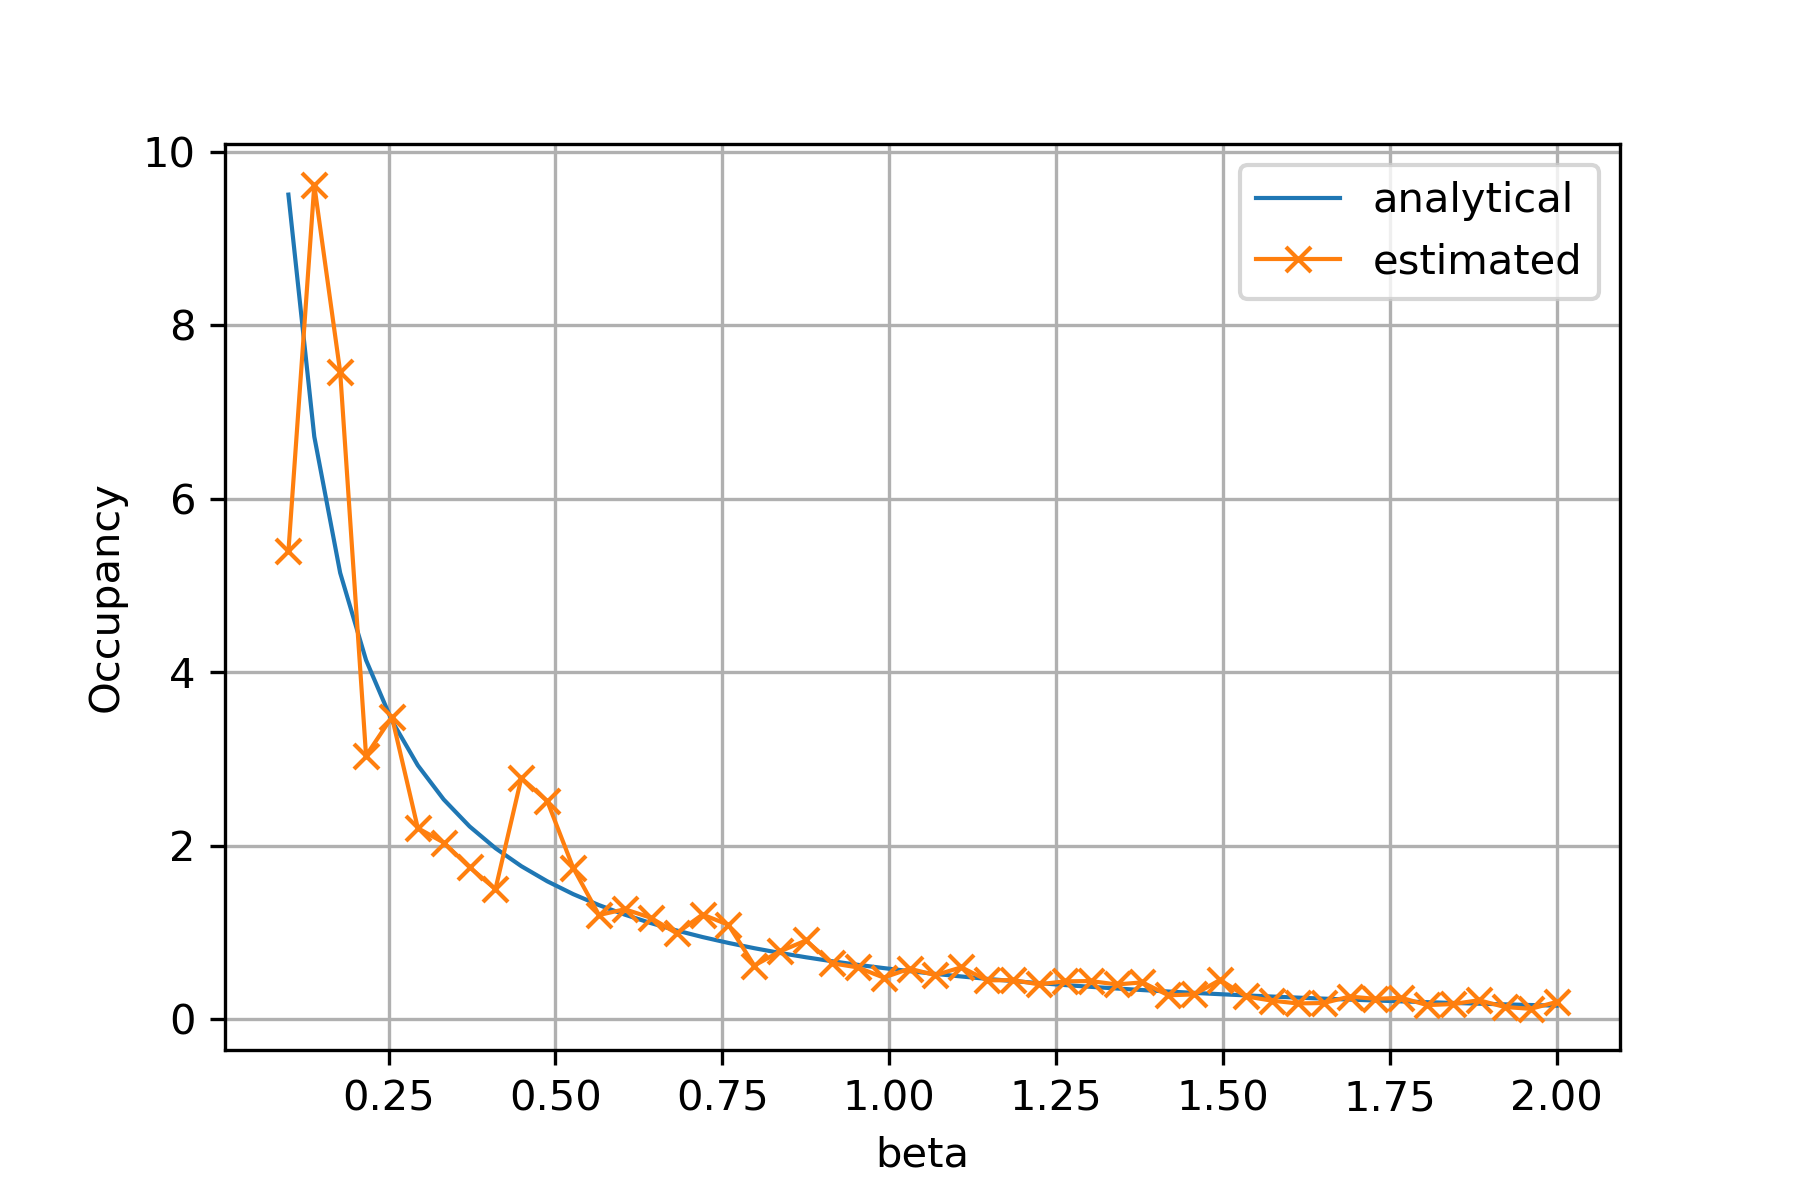
\includegraphics[width=0.6\linewidth]{photon_distribution.png}		
			\caption{Photon-distribution analytical and calculated.}
			\label{fig::noDegeneracy}
		\end{figure}  
		
		We observe that our approximation fits better as beta gets larger. This means that for small values of $\beta$, the error of the estimated average occupancy with respect to the true value is larger. That is what was expected since small $\beta$ implies a high $T$, which means all particles are moving around; hence, it is hard to predict what their occupancy is. As $\beta$ gets smaller, all particles tend to their equilibrium positions. 
		
		\item
		**Bonus:** Modify the program in such a way that the averages are updated only after an accepted trial move. Why does ignoring rejected moves lead to erroneous results? Starting from $P_{acc} ( o \rightarrow n)$, define $P'(o \rightarrow o)$ (*i.e*	the probability that you stay in the old configuration). Recall that
		the transition probability $P'$ is normalised.
		
		Deriving the total energy of an idealised photon gas from quantum mechanics, we know that $U$ can be	written as the sum of the harmonic oscillation energies:
		
		$$
		\begin{aligned}
		U= \sum_{j=1}^{N} n_j w_j \hbar = \sum_{j=1}^{N} n_j \epsilon_j,
		\end{aligned}
		$$
		
		with $\left<n_j\right>$ the ensemble average of the state occupancy.
		
		Thus, if we update both the number of visited states and sum over all occupations a trial move after accepting the trial move only, ergodicity is not fulfilled since we do not consider those states that result in an energy increase of the system. In addition, we can say that the sample space does not include all accessible configurations and then the computed probability is incorrect.  


	\end{enumerate}
  
  \section*{Sampling Configurational Space}
  
  \begin{enumerate}
  	\item 
  	Perform a simulation at $T = 2.0$ and $\rho \in 0.05, 0.2, 0.5, 1$ for 10000 steps with maximum displacement of 0.1 by executing all the cells until but not including the **Visualization of results** block. What do you observe? Check the energies that are printed for the steps. It is not necessary to plot the energies.

  	When $\rho = 0.05$, the energy of the system remains close to a specific value.
	
	When $\rho = 0.20$, the energy of the system varies largely and it keeps increasing after we consider larger number of steps. That is, for 1000 steps the energy is -262.72 and for 9000 the energy is -680.37. We have the same behavior when we use $\rho = 0.5$, but in this case, the energy variation is even larger: for 1000 steps the energy is -377.68 and for 9000 the energy is -2787.63.
	
	On the other hand, when $\rho = 1$, although the energy varies at the first steps, it reaches a steady value or level and it stays remains close to such a level when increasing the number of steps.	

  	\item 
  	Is it justified to assume non-interacting Lennard Jones particles for all values of $\rho$?	
  
  	When varying $\rho$, it means that particles are either closer or farther away from each other since we keep constant both volume of and number of particles of the system. As a result, for large values of $\rho$, which correspond to the density of the particles, it should be erroneous to consider that particles are not interacting since they are really close to each other. However, when using small values of $\rho$, we could assume non-interacting particles.
 
  	\item
  	The program produces a sequence of snapshots of the state of the system as xyz file. You can visualise them directly in the notebook. Explain the behaviour of the system for frame 0, 1000, 5000 and 9000 for $\rho=0.4$
  	
  	We have the following plots: 
  	  	
  	\begin{figure}[H]
  		\centering
  		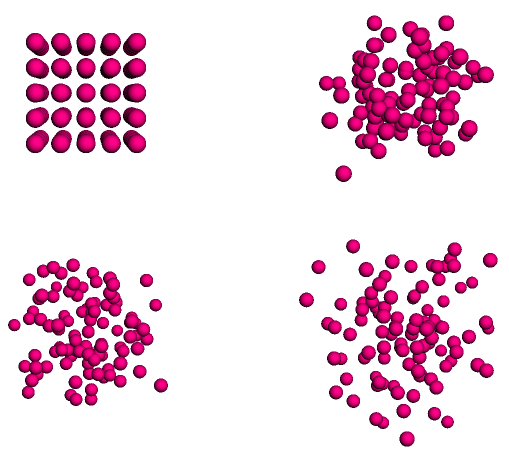
\includegraphics[width=0.5\linewidth]{SamplingConfigurational3.png}		
  		\caption{System's behavior}
  		\label{fig::SamplingConfigurational_3}
  	\end{figure} 
  	  	
  	When increasing the number of steps (simulation time), the particles are father away from each other. 
  	We can think of this as the particles are interacting with each other for the total length of the simulation. Given the snapshots, we can stay that the system is in the repulsion zone of the Lennard Jones potential or that the particles repulse each other. Additionally, we may say that the system has not reached equilibrium and more simulation steps are required; the Monte Carlo method works for systems that have reached the invariant distribution. 
  	
  	If we ran the simulation for a larger number of steps, we would probably observe the particles reaching their equilibrium states, which means particles not changing largely their positions.
  	
	\item
	Instead of performing a trial move in which only one particle is displaced, one can do a trial move in which all particles are displaced. What do you expect will happen to the maximum displacements of these moves for a fixed acceptance rate of all displacements (for example 50\%)?
	
	If $\Delta \text{displacement}$ is large, it is likely that the resulting configuration will have a high energy and the trial move will rejected most of time. If it is very small, the change of potential energy is probably small and many moves will be accepted. 
	
	Besides, there is a rule of thumb which states that an acceptance of approximately 50\% should be optimal. However, the optimum acceptance ratio is the one that leads to the most efficient sampling of configuration space. It makes a important difference if the the computational resources required to test a trail move is accepted depends on the size of the move. In the Metropolis algorithm, all interactions are computed before accepting or rejecting and then the computational cost does not depend on the size of the trial move. On the other hand, for molecules with hard repulsive cores, a move can be rejected as soon as an overlap with any neighbor is detected. In this case, a rejected move is cheaper than an accepted one.
	
	As a result, we can expect that the parameter $\Delta \text{displacement}$ is adjusted in such a way that it will not be either too large or too small; then the the evolution of the system with MC steps will reach an invariant distribution.
	
	\item 
  	**Bonus** Describe the changes in the code to sample from the isothermic-isobaric ensemble (NpT) instead of the microcanonical ensemble (NVT)?
  	
  	In the NVT ensemble volume is allowed to vary then a Markov chain must be constructed in which both particle moves
  	and volume changes are allowed. It is important to mention that a change in volume implies a change in particle positions. Therefore, a change of volume must be followed by a proper re-scaling of particle positions. 
  	
  	A simulation step consists of either a particle move, which is performed exactly like the particle moves in the NVT ensemble, or a volume change. The calculation of the ratio of the weights before and after the volume change consists of calculating the change due to the potential energy given by:    	
  	
  	Besides, the Boltzmann weight of NVT ensemble is replaced by:
  	$$
  	e^{-\beta P V }\cdot V^{N} \cdot e^{-\beta U(L) }
  	$$
  	
  	To compute the ratio of the weights before and after the volume change, it consists of calculating the change due to the potential energy: 
  	
  	$$
  	\text{exp}\left[ -\beta \left( U(L_{new})  - U (L_{old}) \right) \right]  	
  	$$
  	
  	And considering the ratio of terms related to the volume coordinate, we have: 
  	
  	$$
  	\text{exp}\left[ -\beta P(V_{new} - V_{old}) \right]
  	\cdot  \left( \dfrac{V_{new}}{V_{old}}\right)^{N}
  	$$
  	
  	Hence, the acceptance ratio of the new configuration according to the Metropolis algorithm is the product of these quantities: 
  	
  	$$
  	\text{exp}\left[ -\beta \left( U(L_{new})  - U (L_{old}) \right) \right]  
  	\cdot
  	\text{exp}\left[ -\beta P(V_{new} - V_{old}) \right]
  	\cdot  \left( \dfrac{V_{new}}{V_{old}}\right)^{N}
  	$$        	
  	  
  \end{enumerate}

\end{document}    